\documentclass[12pt]{article}
\usepackage{amsthm,amssymb,amsfonts,amsmath,amstext,systeme,xcolor, stix,graphicx,float}
\usepackage{graphicx,float}
\newcommand\norm[1]{\lVert#1\rVert}
\marginparwidth0pt
\oddsidemargin -1.4 truecm
\evensidemargin0pt
\marginparsep0pt
\topmargin -2.5truecm
\textheight 26.3truecm
\textwidth 18.9 truecm
\linespread{1.3}
\newtheorem{theorem}{Theorem}[section]
\newtheorem{lemma}[theorem]{Lemma}
\newtheorem{corollary}[theorem]{Corollary}
\newtheorem{proposition}[theorem]{Proposition}
\newenvironment{remark}{\noindent{\bf Remark}}{\vspace{3mm}}
\newenvironment{remarks}{\noindent{\bf Remarks }}{\vspace{0mm}}
\newenvironment{notes}{\noindent{\bf Notes}}{\vspace{0mm}}
\newenvironment{note}{\noindent{\bf Note}}{\vspace{0mm}}
\newenvironment{solution}{\noindent{\it Solution\/}}{\vspace{2mm}}
\newenvironment{question}{\noindent{\bf Question}}{\vspace{0mm}}
\newenvironment{questions}{\noindent{\bf Questions}}{\vspace{0mm}}
\newenvironment{example}{\noindent{\bf Example }}{\vspace{0mm}}
\newenvironment{examples}{\noindent{\bf Examples }}{\vspace{0mm}}
\newcommand{\ds}{\displaystyle}
\newcommand{\bs}{\boldsymbol}

\begin{document}

\begin{center}
\vspace{0.6cm}
{\Large \bf To-Do List Year 2 Fall Semester}
\vspace{0.3cm}
\end{center}

\section{Chapter 1}
\subsection{System of Linear Equation}
A system of linear Equations has
\begin{enumerate}
    \item no solution, or
    \item exactly one solution, or
    \item infinitely many solutions
\end{enumerate}
Definition: If there is no solution exist, we say the linear system is inconsistent, otherwise, the linear system is consistent

\subsection{Row Reduction and Echelon forms}
\begin{enumerate}
    \item Each matrix is row equivalent to one and only one reduced echelon matrix.
    \item Columns contain leading 1(pivot position) are pivot columns.
    \item From matrix to echelon form is forward phase while from echelon form to reduced echelon form called backward phase.
    \item Variables in linear systems can be divided as basic and free variables(free to choose any value).
\end{enumerate}
\subsection{Vector Equations}
Linear Combinations: In general, given vectors $\vec{v_1}, \vec{v_2}, \cdots, \vec{v_p}$ in $\mathbb{R}^n$, and given scalars $C_1, C_2, \cdots, C_p$, the vector $\vec{w}$\\
$\vec{w} = C_1 \vec{v_1} + C_2 \vec{v_2} + \cdots + C_p \vec{v_p}$ with weights coefficients $C_1, C_2, \cdots, C_p$. 

Definition: If $\vec{v_1}, \vec{v_2}, \cdots, \vec{v_p}$ are vectors in $\mathbb{R}^n$, then the set of all linear combinations of $\vec{v_1}, \vec{v_2}, \cdots, \vec{v_p}$ is denoted by span$\{\vec{v_1}, \vec{v_2}, \cdots, \vec{v_p}\}$ and is called {\bf the subset of }$\mathbb{R}^n${\bf (or generated) by }$\vec{v_1}, \vec{v_2}, \cdots, \vec{v_p}$.

That is, span$\{\vec{v_1}, \vec{v_2}, \cdots, \vec{v_p}\}$ is the collection of all vectors that can be written in the form $\vec{w} = C_1 \vec{v_1} + C_2 \vec{v_2} + \cdots + C_p \vec{v_p}$. 

\subsection{The matrix Equation $A\vec{x} = \vec{b}$}
Let $A$ is an $m \times n$ matrix, the following statements are equivalent:
\begin{enumerate}
    \item For each $\vec{b}$ in $\mathbb{R}^m$, the equation $A\vec{x} = \vec{b}$ has a solution.
    \item Each $\vec{b} \in \mathbb{R}^m$ is a linear combination of the column vectors of $A$.
    \item The column vectors of $A$ span $\mathbb{R}^m$.
    \item $A$ has a pivot position in every row.
\end{enumerate}
\subsection{Solution Sets of Linear Systems}

Homogenous Linear Systems: $$A\vec{x} = \vec{0}$$

It always has a trivial solution $\vec{x} = \vec{0}$
The system $A\vec{x} = \vec{0}$ has nontrivial solution if and only if the system has at least one free variable.

Parametric Vector Form: $$\vec{x} = s\vec{u} + t\vec{v}\text{ where } s,t \in \mathbb{R}$$

Theorem: Suppose $A\vec{x} = \vec{b}$ is consistent for some given $\vec{b}$ and let $\vec{p}$ be a solution. Then the solution set of $A\vec{x} = \vec{b}$ is the set of all vectors of the form $\vec{w} = \vec{p} + r\vec{v_n}$, there $\vec{v_n}$ is any solution of $A\vec{x} = \vec{0}$.


Remarks: Describe the free variables as arbitrary.

A set of vectors $\{\vec{v_1}, \vec{v_2}, \cdots, \vec{v_p}\}$ in $\mathbb{R}^n$ is said to be {\bf Linear Independent} if the vector equation $C_1 \vec{v_1} + C_2 \vec{v_2} + \cdots + C_p \vec{v_p} = \vec{0}$ has only the trivial solution. 

\subsection{Linear Independent}
The column vectors of a matrix $A$ are {\bf Linearly Independent} if and only if $A\vec{x} = \vec{0}$ has only the trivial solution.

Sets of One or Two Vectors:
\begin{enumerate}
    \item $\{\vec{v}\}$ is linearly independent if and only if $\vec{v} \neq \vec{0}$
    \item $\{\vec{v_1}, \vec{v_2}\}$ is linearly independent if and only if neither of the vectors is a multiple of the other $\iff$ $\{\vec{v_1}, \vec{v_2}\}$ is linearly dependent if at least one of the vectors is a multiple of the other, where the constant can be 0.
\end{enumerate}

Characterization of linearly dependent sets:
$\{\vec{v_1}, \vec{v_2}, \cdots , \vec{v_p}\}$ where $p\geq 2$ is linearly dependent if and only if at least one of the vectors is a linear combination of the others.

Theorem: If $\{\vec{v_1}, \vec{v_2}, \cdots , \vec{v_p}\}$ where $p\geq 2$, $\vec{v_1}, \vec{v_2}, \cdots , \vec{v_p}$ are vectors in $\mathbb{R}^n$. If ${P>n}$, then $\{\vec{v_1}, \vec{v_2}, \cdots , \vec{v_p}\}$ must be {\bf Linearly Dependent}.

\subsection{Introduction to Linear Transformations}
Definition: A transformation from $\mathbb{R}^n$ to $\mathbb{R}^m$, $T: \mathbb{R}^n  \longmapsto  \mathbb{R}^m$ is a rule that assigns to each vector in $\mathbb{R}^n$ to a vector $T(\vec{x})$ in $\mathbb{R}^m$.
\begin{enumerate}
    \item[$\mathbb{R}^n$ :] {\bf Domain} of $T$.
    \item[$\mathbb{R}^n$ :] {\bf Codomain} of $T$.
\end{enumerate}
For $\vec{x}\in \mathbb{R}^n$, $T(\vec{x})$ is called the image of $\vec{x}$. The set of all images $T(\vec{x})$ is called the range of $T$.

Definition: A transformation (or mapping) $T$ is {\bf linear} if 
\begin{enumerate}
    \item $T(\vec{u}+\vec{v}) = T(\vec{u}) + T(\vec{v})$ for all $\vec{u}, \vec{v} \in D(T)$ of $T$
    \item $T(c\vec{u}) = cT(\vec{u})$ for all scalars $c$ and $\vec{u} \in D(T)$.
    \item $T(\vec{0}) = \vec{0}$
\end{enumerate}


\subsection{The Matrix of a Linear Transformation}
Theorem: Let $T: \mathbb{R}^n  \longmapsto  \mathbb{R}^m$ be a linear transformation. Then there exists a unique matrix $A$ such that $T(\vec{x}) = A\vec{x}$ for all $\vec{x}$ in $\mathbb{R}^n$.

Definition: 
\begin{enumerate}
    \item A map $T: \mathbb{R}^n  \longmapsto  \mathbb{R}^m$ is said to be \textcolor{red}{onto} $\mathbb{R}^m$ if each $\vec{b}$ in $\mathbb{R}^m$ is the image of at least one $\vec{x}$ in $\mathbb{R}^n$.
    \item A map $T: \mathbb{R}^n  \longmapsto  \mathbb{R}^m$ is said to be \textcolor{red}{one-to-one} if $T\vec{x} = T\vec{y}$, then $\vec{x} = \vec{y}$, i.e. each $\vec{b}$ in $\mathbb{R}^m$ is the image of at most one $\vec{x}$ in $\mathbb{R}^m$.
\end{enumerate}

Theorem: Let $T: \mathbb{R}^n  \longmapsto  \mathbb{R}^m$ be a linear transformation. Then $T$ is \textcolor{red}{one-to-one} if and only if the equation $T\vec{x} = \vec{0}$ has only the trivial solution.


Theorem: Let $T: \mathbb{R}^n  \longmapsto  \mathbb{R}^m$ be a linear transformation, and let $A$ be the standard matrix of $T$. 
\begin{enumerate}
    \item $T$ maps $\mathbb{R}^n$ onto $\mathbb{R}^m$ iff the column vectors of $A$ span $\mathbb{R}^m$.
    \item $T$ is one-to-one iff the column vectors of $A$ are linear independent.
\end{enumerate}


Remarks: Column of $A$ does not span $\mathbb{R}^3$ and $T$ is not onto if there are no solution.




\section{Chapter 2}
\subsection{Matrix Operation}
$A\cdot(B\vec{x})$ is a linear transformation from $\mathbb{R}^n$ to $\mathbb{R}^m$


\subsection{The Inverse of Matrix}
Definition: An $n\times n$ matrix $A$ is said to be \textcolor{red}{invertible} if there is an $n\times n$ matrix $C$ such that $$CA = I_n \text{ and }AC = I_n$$

In this case, $C$ is an inverse of $A$ and denoted by $A^{-1}$
Remark: The inverse of $A$ is unique.

Definition: If a matrix is not invertible, it is called singular matrix.

Theorem: Let $\begin{pmatrix}
a & b \\
c & d 
\end{pmatrix}$. If $ad-bc\neq 0$, then $A$ is invertible and $A^{-1} = \dfrac{1}{ad-bc}\begin{pmatrix}
    d&-b\\
    -c&a
\end{pmatrix}$. If $ad-bc = 0$, then $A$ is not invertible and $ad-bc $ is called the determinant of $A$, denoted by det$(A)$

Theorem:
\begin{enumerate}
    \item If $A$ is invertible matrix, then $A^{-1}$ is invertible and $(A^{-1})^{-1} = A$.
    \item If $A$ and $B$ are $n\times n$ invertible matrices, then so is $AB$, and the increase of $A$ and $B$ in the reverse order. That is, $$(AB)^{-1} = B^{-1}A^{-1}$$
    \item If $A$ is an invertible matrix, then so is $A^T$, and the inverse of $A^T$ is the transpose of $A^{-1}$. That is, $$(A^T)^{-1} = (A^{-1})^T$$
\end{enumerate}

Theorem: An $n \times n$ matrix $A$ is invertible iff $A$ is row equivalent to $I_n$, and this case, any sequence of elementary row operations that reduces $A$ to $I_n$ also transform $I_n$ into $A^{-1}$.

Find the third column of $A^{-1}$ without computing the other columns.
$[A\text{    } e_3 ]\sim [I \text{    }b_3]$


\subsection{The Characterization of Invertible Matrices}
Theorem: Let $A$ be an $n\times n$ matrix. Then the following statements are equivalent.
\begin{enumerate}
    \item $A$ is an invertible matrix
    \item $A$ is row equivalent to the $n\times n$ identity matrix
    \item $A$ has $n$ pivot positions
    \item The equation $A\vec{x} = \vec{0}$ has only the trivial solution
    \item The columns of $A$ form a linearly independent set.
    \item The linear transformation $\vec{x} \longmapsto A\vec{x}$ is one-to-one.
    \item The equation $A\vec{x} =\vec{b}$ has at least one solution for each $\vec{b}$ in $\mathbb{R}^n$.
    \item The columns span $\mathbb{R}^n$.
    \item The linear transformation $\vec{x} \longmapsto A\vec{x}$ maps $\mathbb{R}^n$ onto $\mathbb{R}^n$.
    \item There is an $n \times n$ matrix $C$ such that $CA = I$.
    \item There is an $n \times n$ matrix $D$ such that $AD = I$.
\end{enumerate}


Method to check whether $A$ is invertible: use row operations to see the number of pivot position whether is equal to $n$.


\section{Chapter 3}
\subsection{Introduction to Determinant}
Theorem: If $A$ is a triangular matrix, then det$(A)$ is the product of the entries on the main diagonal of $A$. 


\subsection{Properties of Determinant}
Theorem:
\begin{enumerate}
    \item If a multiple of one row of $A$ is added to another row to produce a matrix $B$, then $\text{det}B = \text{det}A$.
    \item If two rows of $A$ are interchanged to produce $B$, then $\text{det}B = -\text{det}A$.
    \item If one row of $A$ is multiplied by $k$ to produce $B$, then $\text{det}B = k\cdot\text{det}A$
\end{enumerate}

Theorem: A square matrix $A$ is invertible if and only if $\text{det}A \neq 0$.
\\
\textcolor{red}{Corollary}: $\text{det}A=0$ if the rows of $A$ are linearly dependent

Theorem: 
\begin{enumerate}
    \item $\text{det}A^T = \text{det}A$
    \item Multiplicative Property: $\text{det}(AB) = \text{det}A\cdot\text{det}B$
    \item $\text{det}(A^{-1}) = \dfrac{1}{\text{det}(A)}$
\end{enumerate}
Remark:$\text{det}(A+B) \neq \text{det}A+\text{det}B$


\subsection{Cramer's Rule, Volume, and Linear Transformations}
Theorem: Cramer's Rule
\\
Let $A$ be an invertible $n\times n$ matrix. For any $\vec{b}$ in $\mathbb{R}^n$, the unique solution $\vec{x}$ of $A\vec{x} = \vec{b}$ has entries given by $$\vec{x_i} = \dfrac{\text{det}A_i(b)}{\text{det}A}, i = 1,2,\cdots,n$$

\textcolor{purple}{Determinants as Area or Volume}:
\\
Theorem: If $A$ is a $2\times2$ matrix, the area of the parallelogram determined by the columns of $A$ is $|\text{det}A|$. If $A$ is $3\times3$ matrix, the volume of the parallelepiped determined by the columns of $A$ is $|\text{det}A|$.


\textcolor{purple}{Linear Transformations}:
\\
Theorem: 
\begin{enumerate}
    \item Let $T: \mathbb{R}^2  \longmapsto  \mathbb{R}^2$ be the linear transformation determined by a $2\time2$ matrix $A$. If $s$ is a parallelogram in $\mathbb{R}^2$, then $$\{\text{area of }T(S)\} = |\text{det}A|\cdot \{\text{area of }S\}$$
    \item If $T$ is determined by a $3\times3$ matrix $A$, and if $S$ is a parallelepiped in $\mathbb{R}^3$, then $$\{\text{volume of }T(S)\} = |\text{det}A|\cdot \{\text{volume of }S\}$$
\end{enumerate}



\section{Chapter 4}
\subsection{Vector Spaces and Subspaces}
Definition: A vector space is a nonempty set $V$ of objects, called \textcolor{red}{vectors}, on which are defined two operations, called \textcolor{red}{addition} and \textcolor{red}{multiplication by scalars (real numbers)}, subject to the ten axioms (or rules) listed below. The axioms must hold for all vectors $\vec{v}, \vec{u} \text{ and }\vec{w}$ in $V$ and for all scalars $c$ and $d$.
\begin{enumerate}
    \item The sum of $\vec{u}$ and $\vec{v}$, denoted by $\vec{u} + \vec{u}$, is in $V$.
    \item $\vec{u} + \vec{v} = \vec{v} + \vec{u}$
    \item $(\vec{u} + \vec{v}) + \vec{w} = \vec{u} + (\vec{v} + \vec{w})$
    \item There is a zero vector $\vec{0}$ in $V$ such that $\vec{u} + \vec{0} = \vec{0} + \vec{u} = \vec{u}$
    \item For each $\vec{u}$ in $V$, there is a vector $-\vec{u}$ in $V$ such that $\vec{u} + (-\vec{u}) = \vec{0}$
    \item The scalar multiple of $\vec{u}$ by $c$, denoted by $c\vec{u}$, is in $V$.
    \item $c(\vec{u} + \vec{v}) = c\vec{u} + c\vec{v}$
    \item $(c+d)\vec{u} = c\vec{u} + d\vec{u}$
    \item $c(d\vec{u}) = (cd)\vec{u}$
    \item $1\cdot\vec{u} = \vec{u}$
\end{enumerate}


\textcolor{purple}{Subspaces}:
\\
Definition: A subspace of a vector space $V$ is a subset $H$ of $V$ that has three properties: 
\begin{enumerate}
    \item The zero vector of $V$ is in $H$. ($\vec{0} \in H$)
    \item $H$ is closed under vector addition. That is, for each $\vec{u}$ and $\vec{v}$ in $H$, the sum $\vec{u} + \vec{v}$ is in $H$
    \item $H$ is closed under multiplication by scalars. That is, for each $\vec{u}$ in $H$ and each scalar $c$, the vector $c\vec{u}$ is in $H$.
\end{enumerate}
An equivalent definition, $H$ is a subspace of $V$ if and only if for $\vec{u}$ and $\vec{v}$ in $H$ and any scalar $a$ and $b$, $a\vec{u} + b\vec{v}$ is in $H$.


For every vector spaces $V$, the subsets $V$ and $\{0\}$ are subspaces. Other subspaces are called \textcolor{red}{proper subspaces}.

\subsection{Null Spaces, Column Spaces and Linear Transformation}
\textcolor{purple}{The Null space of a matrix}:
\\
Definition: The null space of an $m\times n$ matrix $A$, written as Null$A$, is the set of all solutions of the homogeneous equation $A\vec{x} = \vec{0}$. In set notation: $$\text{Nul}A = \{\vec{x} : \vec{x} \text{ is in }\mathbb{R}^n \text{ and } A\vec{x} = \vec{0}\}$$
\\
Null$A$ is the set of all $\vec{x} \in \mathbb{R}^n$ that are mapped into the zero vector of $\mathbb{R}^m$ via the linear transformation $\vec{x}  \longmapsto  A\vec{x}$.
\\
Theorem: The null space of an $m\times n$ matrix $A$ is a subspace of $\mathbb{R}^n$.
\\
Remark: When Nul$A$ contains nonzero vectors, the number of vectors in the spanning set for Nul$A$ equals the number of free variables in the equation $A\vec{x} = \vec{0}$.
\\
\textcolor{purple}{The Column space of a matrix}:
\\
Definition: The column space of an $m\times n$ matrix $A$, written as Col$A$, is the set of all linear combinations of the columns of $A$. If $A = [\vec{a_1}, \cdots, \vec{a_n}]$, then  $$\text{Col}A = \text{Span}\{\vec{a_1}, \cdots, \vec{a_n}\} = \{\vec{b}|\vec{b} = A\vec{x} \text{ for some }\vec{x}\text{ in }\mathbb{R}^n\}$$
\\
Theorem: The column space of an $m\times n$ matrix $A$ is a subspace of $\mathbb{R}^m$.
\\
The column space of an $m\times n$ matrix $A$ is all of $\mathbb{R}^m$ if and only if the equation $A\vec{x} = \vec{b}$ has a solution for each $\vec{b}$ in $\mathbb{R}^m$.
\\
Remark: to test a vector in Col$A$ or not, we solve $[A, \vec{u}]$ and see whether $A\vec{x} = \vec{u}$ has a solution. Thus $\vec{u}$ is in Col$A$.

\textcolor{purple}{Contrast Between Nul$A$ and Col$A$ for an $m\times n$ Matrix $A$}:

$$\begin{array}{|c|c|}
    \hline
    \text{Nul}A & \text{Col}A\\
    \hline
    \text{Nul}A\text{ is a subspace of }\mathbb{R}^n & \text{Col}A\text{ is a subspace of }\mathbb{R}^m\\
    \text{Solve }A\vec{x} = \vec{0} \text{ to get Nul}A & \text{Span}\{\vec{a_1}, \cdots, \vec{a_n}\}\\
    \vec{v}\in \text{ Nul}A \iff A\vec{u} = \vec{0} & \vec{u}\in\text{ Col}A \iff A\vec{x} = \vec{u} \text{ consistent}\\
    \hline
\end{array}$$

\textcolor{purple}{Kernel and Range of a Linear Transformation}:
\\
Definition: A linear transformation $T$ from a vector space $V$ into a vector space $W$ is a rule that assigns to each vector $\vec{x}$ in $V$ a unique vector $T(\vec{x})$ in $W$, such that $T(a\vec{u} + b\vec{v}) = aT(\vec{u}) + bT(\vec{v})$ for all vectors $\vec{u}$ and $\vec{v}$ in $V$ and all scalars $a$, $b$.

\textcolor{red}{Kernel (or Null space) of $T$} = $\{\vec{u}\in V | T(\vec{u}) = \vec{0}\}$

\textcolor{red}{Range of $T$} = $\{\vec{w}\in W | \vec{w} = T(\vec{u}) \text{ for some }\vec{u}\in V\}$


\subsection{Linearly Independent Sets, Bases}
Definition: An indexed set of vectors $\{\vec{v_1}, \cdots, \vec{v_p}\}$ in $V$ is said to be \textcolor{red}{linearly independent} if the vector equation $C_1 \vec{v_1} + C_2 \vec{v_2} + \cdots + C_p \vec{v_p} = \vec{0}$ has only trivial solution $C_1 = 0, \cdots , C_p = 0$.

Definition: Let $H$ be a subspace of a vector space $V$. An indexed set of vectors $B = \{\vec{b_1}, \cdots, \vec{b_p}\}$ in $V$ is a \textcolor{red}{basis} for $H$ if 
\begin{enumerate}
    \item $B$ is a linearly independent set, and
    \item the subspace spanned by $B$ coincides with $H$. That is, $H =\text{ Span}\{\vec{b_1}, \cdots, \vec{b_p}\}$
\end{enumerate}

Example: $A$: $n\times n$ matrix, $A = \{\vec{a_1}, \cdots, \vec{a_n}\}$

If $A$ is invertible ($\text{det}A \neq 0$), then $\vec{a_1}, \cdots, \vec{a_n}$ are linearly independent, $\vec{b} = A\vec{x}$ always has a solution $\vec{x} = A^{-1}\vec{b}$. Thus $\mathbb{R}^n =\text{ Span}\{\vec{a_1}, \cdots, \vec{a_n}\}$  is a basis of $\mathbb{R}^n$

Observation:
\begin{enumerate}
    \item Each non-pivot column of $B$ is a linear combination of the pilot columns. 
    \item If $A$ is a matrix whose reduced echelon form is $B$, then $A\vec{x} = \vec{0}$ iff $B\cdot \vec{x} = \vec{0}$
\end{enumerate}

Theorem: The pivot columns of a matrix $A$ form a basis for Col$A$.

\subsection{Coordinate Systems}
Theorem: The Unique Representation Theorem

Let $B = \{\vec{b_1}, \cdots, \vec{b_n}\}$ be a basis for a vector space $V$. Then for each $\vec{x}$ in $V$, there exists a unique set of scalars $C_1, C_2, \cdots, C_n$ such that $$\vec{x} = C_1\vec{b_1}+\cdots + C_n\vec{b_n}$$

Theorem: Let $B = \{\vec{b_1}, \cdots, \vec{b_n}\}$ be a basis for a vector space $V$. Then the coordinate mapping $\vec{x} \longmapsto [\vec{x}]_B$ is a one-to-one linear transformation from $V$ onto $\mathbb{R}^n$. And the transformation is called \textcolor{red}{isomorphism}.
\subsection{The Dimension of a Vector Space}
Theorem: If a vector space $V$ has a basis $B = \{\vec{b_1}, \cdots, \vec{b_n}\}$, then any set in $V$ containing more than $n$ vectors must be linearly dependent.

Theorem: If a vector space $V$ has a basis of $n$ vectors, then every basis of $V$ must consist of exactly $n$ vectors.

Definition: If $V$ is spanned by a finite set, then $V$ is said to be \textcolor{red}{finite-dimensional}, and the dimension of $V$, written as dim$V$, is the number of vectors in a basis for $V$. The dimension of the zero vector space $\{\vec{0}\}$ is defined to be zero. If $V$ is not spanned by a finite set, then $V$ is said to be \textcolor{red}{infinite-dimensional}.

\textcolor{purple}{Subspace of a Finite-Dimensional Space}:
Theorem: Let $H$ be a subspace of a finite-dimensional vector space $V$. Any linearly independent set in $H$ can be expanded, if necessary, to a basis for $H$. Also, $H$ is finite-dimensional and $$\text{dim}H \leq \text{dim}V.$$

\textcolor{purple}{The Basis Theorem}:
Let $V$ be a $p$-dimensional vector space, $p \geq 1$, any linearly independent set of exactly $p$ elements in $V$ is automatically a basis for $v$. Any set of exactly $p$ elements that spans $V$ is automatically a basis for $V$.

\textcolor{purple}{The Spanning Set Theorem}:
Let $S = \{\vec{v_1}, \cdots, \vec{v_p}\}$ be a set in $V$, and let $H = \text{Span}\{\vec{v_1}, \cdots, \vec{v_p}\}$.
\begin{enumerate}
    \item If one of the vectors in $S - $ say, $\vec{v_k} - $ is a linear combination of the remaining vectors in $S$, then the set formed from $S$ by removing $\vec{v_k}$ still spans $H$.
    \item If $H \neq \{\vec{0}\}$, some subset of $S$ is a basis for $H$.
\end{enumerate}


\textcolor{purple}{The dimension of Nul$A$ and Col$A$}:
\begin{enumerate}
    \item The dim(Nul$A$) = number of free variables in the equation $A\vec{x} = \vec{0}$
    \item The dim(Col$A$) = number of pivot columns of $A$.
\end{enumerate}


Exercise: Let $V$ is a nonzero finite-dimensional vector space.
\begin{enumerate}
    \item If dim$V = p$ and if $S$ is a linearly dependent subset of $v$, then $S$ contains more than $p$ vectors. Answer: False
    \item If $S$ spans $V$ and if $T$ is a subset of $V$ that contains more vectors than $S$, then $T$ is linearly dependent. Answer: True
\end{enumerate}


\subsection{Rank}
\textcolor{purple}{The Row Space}:
Theorem: The two matrices $A$ and $B$ are row equivalent, then their row spaces are the same.\\
If $B$ is in echelon form, the nonzero rows of $B$ form a basis for the row space of $A$ as well as for that of $B$.

\begin{figure}[H]
    \centering
    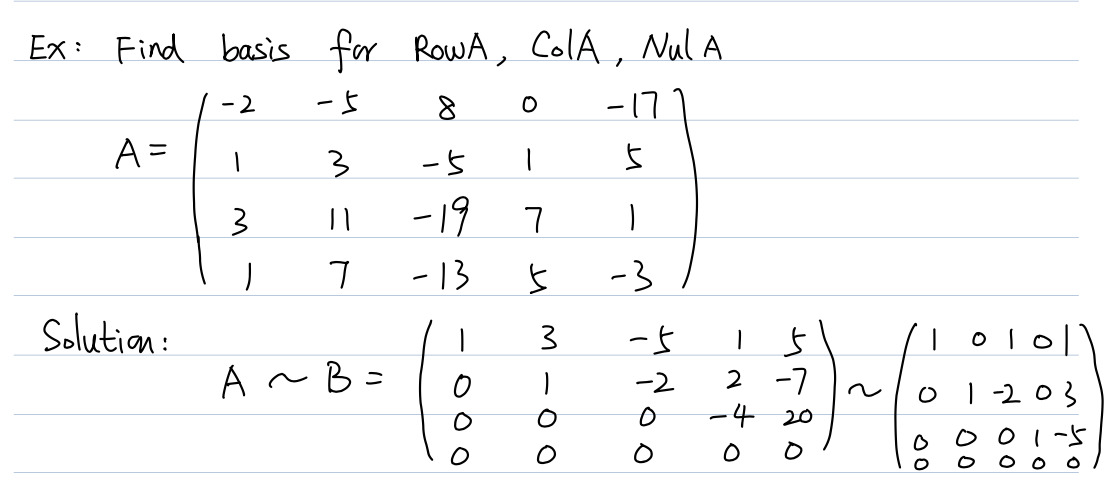
\includegraphics[width = .5\linewidth]{Revision1}
\end{figure}
\begin{figure}[H]
    \centering
    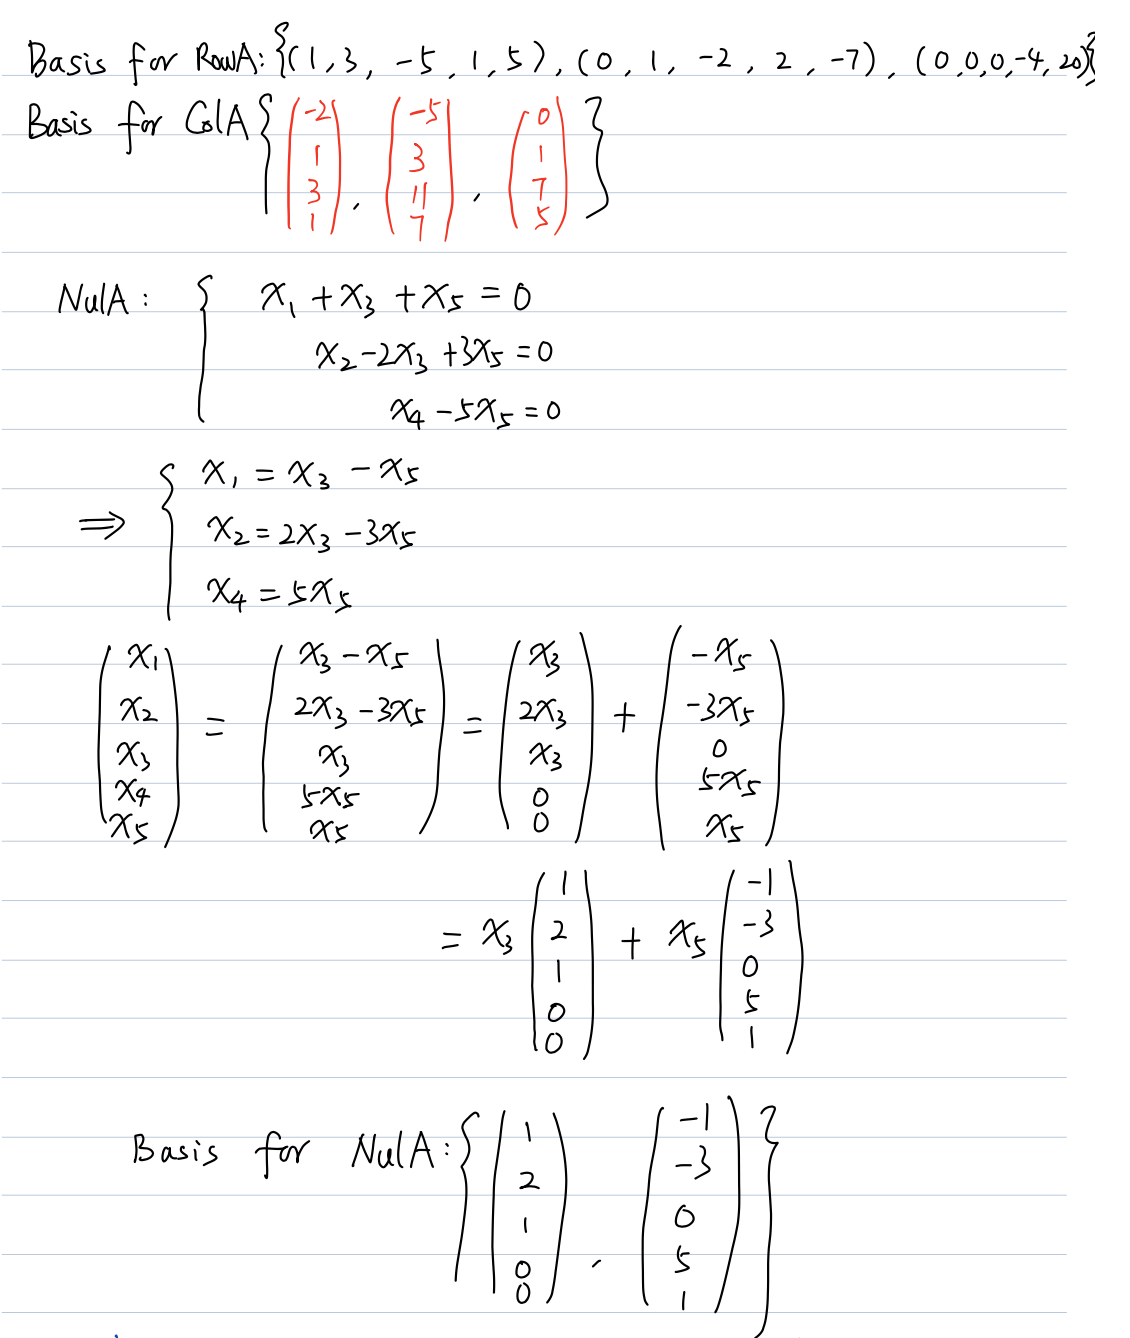
\includegraphics[width = .5\linewidth]{Revision2}
\end{figure}

\textcolor{purple}{The Rank Theorem}:
Definition: The rank of $A$ is the dimension of the column space of $A$.
$$\text{Rank}A = \text{dim}(\text{Col}A)$$

The rank Theorem: Let $A : m\times n$
\begin{enumerate}
    \item $\text{Rank}A = \text{dim}(\text{Col}A) = \text{dim}(\text{Row}A) = \text{number of pivots in }A \leq m $
    \item $\text{Rank}A + \text{dim}(\text{Nul}A = n)$
\end{enumerate}


The Invertible Matrix Theorem:\\
Let $A$ be an $n\times n$ matrix. Then the following statements are equivalent.
\begin{enumerate}
    \item $A$ is an invertible matrix.
    \item $A$ is row equivalent to the $n\times n$ identity matrix.
    \item $A$ has $n$ pivot positions.
    \item The equation $A\vec{x} = \vec{0}$ has only the trivial solution.
    \item The columns of $A$ form a linearly independent set.
    \item The linear transformation $\vec{x}\longmapsto A\vec{x}$ is one-to-one.
    \item The equation $A\vec{x} = \vec{b}$ has at least one solution for each $\vec{b}$ in $\mathbb{R}^n$.
    \item The columns span $\mathbb{R}^n$.
    \item The linear transformation $\vec{x} \longmapsto A\vec{x}$ maps $\mathbb{R}^n$ onto $\mathbb{R}^n$.
    \item There is an $n \times n$ matrix $C$ such that $CA = I$.
    \item There is an $n \times n$ matrix $D$ such that $AD = I$.
    \item $A^T$ is an invertible matrix.
    \item The columns of $A$ form a basis of $\mathbb{R}^n$.
    \item Col$A$ = $\mathbb{R}^n$
    \item dim(Col$A$) = $n$
    \item rank$A$ = $n$
    \item Nul$A$ = $\{\vec{0}\}$
    \item dim(Nul$A$) = 0
    \item det($A$) $\neq 0$
\end{enumerate}


Remarks: Col$A^T$ = Row$A$ and Rank$A^T$ = Rank$A$.


\section{Chapter 5}
\subsection{Eigenvectors and Eigenvalues}
Definition: An \textcolor{red}{eigenvector} of an $n\times n$ matrix $A$ is a nonzero vector $\vec{x}$ such that $A\vec{x} = \lambda\vec{x}$ for some scalar $\lambda$. 
\begin{enumerate}
    \item $\lambda$ is called an eigenvalue of $A$.
    \item $\vec{v}$ is called an eigenvector corresponding to $\lambda$.
\end{enumerate}

Theorem: The eigenvalues of a triangular matrix are the entries on its main diagonal.

The scalar $\lambda$ is an eigenvalue if and only if 
\begin{enumerate}
    \item $(A-\lambda I)\vec{x} = \vec{0}$ has a nontrivial solution.
    \item $(A-\lambda I)\vec{x} = \vec{0}$ has a free variable
    \item at least one of the entries on the diagonal of $A-\lambda I$ is zero. (Number of pivots of $A - \lambda I \leq n$)
    \item $\lambda = a_{11}$ or $\lambda = a_{22}$ or $\cdots, \lambda = a_{nn}$
\end{enumerate}

Example: If $\vec{x}$ is an eigenvector of $A$ corresponding to $\lambda$, $A^n\vec{x} = \lambda^n\vec{x}$

Theorem: If $\vec{v_1}, \cdots, \vec{v_r}$ are eigenvectors that correspond to distinct eigenvalues $\lambda_1, \cdots, \lambda_r$ pf am $n\times n$ matrix $A$, then the set $\{\vec{v_1}, \cdots, \vec{v_r}\}$ is linearly independent.$ \implies $ The eigenvectors are linearly independent.


\subsection{The characteristic equation}
Definition: The characteristic equation: $A: n\times n$ matrix $\text{det}(A-\lambda I) = 0$ is called the characteristic equation of $A$. $\text{det}(A-\lambda I)$ is called the characteristic polynomial of $A$, a polynomial of degree $n$ in the variable $\lambda$.

Theorem: $\lambda$ is an eigenvalue of $A$ if and only if $\lambda$ satisfies the characteristic equation $\text{det}(A-\lambda I) = 0$.

Multiplicity: The degree of the corresponding eigenvalue.


\textcolor{purple}{Similarity}
Definition: Let $A, B$ are $n\times n$ matrices.\\
$A$ is similar to $B$ if there exists an invertible matrix $P$ such that $P^{-1}AP = B$ or equivalently, $A = PBP^{-1}$\\
Changing $A$ into $P^{-1}AP$ is called a similarity transformation.

Theorem: If $n\times n$ matrices $A$ and $B$ are similar, then they have the same characteristic polynomial and hence the same eigenvalues (with the same multiplicities).


Warnings:
\begin{enumerate}
    \item The matrices $\begin{pmatrix}
        2 & 1 \\
        0 & 2 
        \end{pmatrix}$ and $\begin{pmatrix}
            2 & 0 \\
            0 & 2 
        \end{pmatrix}$ are not similar even though they have the same eigenvalues.
    \item Similarity is not the same as row equivalence. Row operations on a matrix usually change its eigenvalues.
\end{enumerate}




\subsection{Diagonalization}
If $A = PDP^{-1}$ where $P$ is invertible and $D$ is diagonal, then $A^k = PD^kP^{-1}$.

Definition: A square matrix $A$ is said to be diagonalizable if $A$ is similar to  diagonal matrix. That is, if $A = PDP^{-1}$ for some invertible matrix $P$ and some diagonal matrix $D$.

The Diagonalization Theorem:

An $n\times n$ matrix $A$ is diagonalizable iff $A$ has $n$ linearly independent eigenvectors.

$A = PDP^{-1}$ with $D$ is diagonal matrix iff the columns of $P$ are $n$ linearly independent eigenvectors of $A$. In this case, the diagonal entries of $D$ are eigenvalues of $A$ that correspond, respectively, to the eigenvectors in $P$.


\textcolor{purple}{Diagonalizing Matrices}
\begin{enumerate}
    \item Find eigenvalues: $\text{det}(A-\lambda I) = 0$
    \item Find linearly independent eigenvectors of $A$: $(A-\lambda I)\vec{x} = \vec{0}$
    \item Construct $P$: $P = (\vec{v_1}, \vec{v_2}, \vec{v_3})$
    \item Construct $D$.
\end{enumerate}

Theorem: An $n\times n$ matrix with $n$ distinct eigenvalues is diagonalizable.

\textcolor{purple}{Matrices Whose Eigenvalues Are Not Distinct}:
Theorem: Let $A$ be an $n\times n$ matrix whose distinct eigenvalues are $\lambda_1, \cdots, \lambda_p$.
\begin{enumerate}
    \item For $1\leq k \leq p$, the dimension of the eigenspace for $\lambda_k$ is less than or equal to the multiplicity of the eigenvalue $\lambda_k$.
    \item The matrix $A$ is diagonalizable iff the sum of the dimensions of the eigenspace equals to $n$m and this happens if and only if \begin{enumerate}
        \item The characteristic polynomial factors completely into linear factors
        \item The dimension of the eigenspace for each $\lambda_k$ equals the multiplicity of $\lambda_k$.
    \end{enumerate}
\end{enumerate}


Remarks: 
\begin{enumerate}
    \item If $A = PDP^{-1}$, then $A^{-1} = PD^{-1}P^{-1}$.
    \item If $A = PDP^{-1}$, then $A^{T} = P^TDP^{-1}$.
\end{enumerate}



\subsection{Discrete Dynamical Systems}
\subsection{Applications to Differential Equations}





\section{Chapter 6}
\subsection{Inner Product, Length and Orthogonality}
\textcolor{purple}{The Inner Product}:
$$\vec{a}^T \vec{b} = a_1b_1+a_2b_2+\cdots+a_nb_n= \vec{a} \cdot \vec{b}$$

Theorem: Let $\vec{u}$, $\vec{v}$ and $\vec{w}$ be vectors in $\mathbb{R}^n$, and let $c$ be a scalar. Then
\begin{enumerate}
    \item $\vec{u} \cdot \vec{v} = \vec{v} \cdot \vec{u}$
    \item $(\vec{u}+\vec{v}) \cdot \vec{w} = \vec{u} \cdot \vec{w}+\vec{v} \cdot \vec{w}$
    \item $(c\vec{u})\cdot\vec{v}=c(\vec{u} \cdot \vec{v}) = \vec{u} \cdot (c\vec{v})$
    \item $\vec{u} \cdot \vec{u} \geq 0 and \vec{u} \cdot \vec{u} = 0$ iff $\vec{u} = \vec{0}$
\end{enumerate}

\textcolor{purple}{The length of a vector}:
Definition: The length (or norm) of $\vec{u}$ is the non-negative scalar $\norm{\vec{x}}$ defined by $$\norm{\vec{u}} = \sqrt{\vec{u} \cdot \vec{u}} = \sqrt{\vec{u_1}^2+\vec{u_2}^2+\cdots+\vec{u_n}^2}$$


Unit Vector: $\vec{u} = \dfrac{\vec{v}}{\norm{\vec{v}}}$

\textcolor{purple}{Distance in $\mathbb{R}^n$}:
Definition: For $\vec{u}$ and $\vec{v}$ in $\mathbb{R}^n$, the distance between $\vec{u}$ and $\vec{v}$, written as dist($\vec{u}, \vec{v}$), is the length of the vector $\vec{u}-\vec{v}$. That is, $$\text{dist}(\vec{u}, \vec{v}) = \norm{\vec{u} - \vec{v}}$$


\textcolor{purple}{Orthogonal Vectors(Perpendicular)}:\\
Definition: Two vectors $\vec{u}$ and $\vec{v}$ in $\mathbb{R}^n$ are orthogonal (to each other) if $\vec{u}\cdot\vec{v} =0$.

Remarks: $\vec{0}$ is orthogonal to every vector in $\mathbb{R}^n$ because $\vec{0}^T\vec{0} = 0$


\textcolor{purple}{Orthogonal Complements}:\\
Definition: Let $\vec{z} \in \mathbb{R}^n$, $W$ a subspace of $\mathbb{R}^n$. If $\vec{z}$ is orthogonal to every vector in $W$, we say $\vec{z}$ is orthogonal to $\vec{w}$.

Definition: The set of all vectors $\vec{z}$ that are orthogonal to $W$ is called the orthogonal complement of $W$, and is denoted by $W^\perp$.

Fact:
\begin{enumerate}
    \item A vector $\vec{x}$ is in $W^\perp$ iff $\vec{x}$ is orthogonal to every vector in a set that spans $W$. 
    \item $W^\perp$ is a subspace of $\mathbb{R}^n$.
\end{enumerate}


Theorem: Let $A$ be an $m\times n$ matrix. The orthogonal complement of the row space of $A$ is the null space of $A$, and the orthogonal complement of the column space of $A$ is the null space of $A^T$.
$$(\text{Row}A)^\perp = \text{Nul}A$$
$$(\text{Col}A)^\perp = \text{Nul}A^T$$

Let $W$ be a subspace of $\mathbb{R}^n$. Then $W^\perp$ is also a subspace of $\mathbb{R}^n$.
$$\text{dim}W + \text{dim}W^\perp = n$$







\subsection{Orthogonal Sets}
Definition: A set of vectors $\{\vec{u_1}, \cdots, \vec{u_p}\}$ in $\mathbb{R}^n$ is said to be an orthogonal set if each pair of distinct vectors from the set is orthogonal, that is, if $\vec{u_i}\cdot\vec{u_j} = 0$ whenever $i \neq j$.

Theorem: If $S = \{\vec{u_1}, \cdots, \vec{u_p}\}$ is an orthogonal set of nonzero vectors in $\mathbb{R}^n$, then $S$ is linearly independent and hence is a basis for the subspace spanned by $S$.


Definition: An orthogonal basis for a subspace $S$ of $\mathbb{R}^n$ is a basis for $W$ that is also an orthogonal set.


Theorem: Let $\{\vec{u_1}, \cdots, \vec{u_p}\}$ be an orthogonal basis for a subspace $W$ of $\mathbb{R}^n$. For each $y$ in $W$, the weights in the linear combination $$\vec{y} = C_1 \vec{v_1} + C_2 \vec{v_2} + \cdots + C_p \vec{v_p}$$
are given by $$C_j = \dfrac{\vec{y}\cdot\vec{u_j}}{\vec{u_j}\cdot\vec{u_j}}, j = 1,\cdots, p$$

Remarks: If the basis were not orthogonal, it would be necessary to solve a system of linear equations in older to find the weights.

Orthogonal Projection:
$$\text{Proj}_{\vec{u}} \vec{y} = \dfrac{\vec{u}\cdot\vec{y}}{\vec{u}\cdot\vec{u}}\vec{u} = \dfrac{\vec{u}\cdot\vec{y}}{{\norm{\vec{u}}}^2}\vec{u}$$ 
$$\vec{w} = \vec{y} - \dfrac{\vec{u}\cdot\vec{y}}{\vec{u}\cdot\vec{u}}\vec{u}$$


\textcolor{purple}{Orthonormal Sets}:\\
A set contains unit vectors, i.e. $\vec{u_i} \cdot \vec{u_j} = 0$ for $i \neq j$ and $\vec{u_i} \cdot \vec{u_i} = 1$. If $W$ is a subspace spanned by an orthonormal set, then the set is an orthonormal basis for $W$.

\textcolor{purple}{Orthonormal columns}:\\
Theorem: An $m\times n$ matrix $U$ has orthonormal columns iff $U^TU = I$. 

Theorem: Let $U$ be an $m\times n$ matrix with orthonormal columns, and let $\vec{x}$ and $\vec{y}$ be in $\mathbb{R}^n$. Then
\begin{enumerate}
    \item $\norm{U\vec{x}} = \norm{\vec{x}}$
    \item $(U\vec{x})(U\vec{y}) = \vec{x}\cdot\vec{y}$
    \item $(U\vec{x})(U\vec{y}) = 0$ if and only if $\vec{x}\cdot\vec{y} = 0$. 
\end{enumerate}


Remarks: Properties 1 and 3 say that the linear mapping $\vec{x}\longmapsto U\vec{x}$ preserves lengths and orthogonality.




\subsection{Orthogonal Projection}
In general, find a decomposition of $\vec{u}$ in $\mathbb{R}^n$ as $\vec{u} = \vec{u_1} + \vec{u_2}$, $\vec{u_1}$ is in a subspace $W$ and $\vec{u_2}$ is in $W^\perp$.\\
$\vec{u_1}$ is called the orthogonal projection of $\vec{u}$ onto the subspace $W$.

\textcolor{purple}{The Orthogonal Decomposition Theorem}:\\
Let $W$ be a subspace of $\mathbb{R}^n$. Then each $\vec{y}$ in $\mathbb{R}^n$ can be written uniquely in the form $$\vec{y} = \hat{\vec{y}} + \vec{z}$$
where $\hat{\vec{y}}$ is in $W$ and $\vec{z}$ is in $W^\perp$. In fact, if $\{\vec{u_1}, \cdots, \vec{u_p}\}$ is any orthogonal basis of $W$, then 
$$\hat{\vec{y}} = \dfrac{\vec{u_1}\cdot\vec{y}}{\vec{u_1}\cdot\vec{u_1}}\vec{u_1} + \cdots + \dfrac{\vec{u_p}\cdot\vec{y}}{\vec{u_p}\cdot\vec{u_p}}\vec{u_p}$$
and $\vec{z} = \vec{y} - \hat{\vec{y}}$.


\textcolor{purple}{Properties of Orthogonal Projections}:

Let $W = \text{span}\{\vec{u_1}, \cdots, \vec{u_p}\}$, where $\{\vec{u_1}, \cdots, \vec{u_p}\}$ is an orthogonal basis for $W$.

If $\vec{y} \in W$, then $\text{Proj}_W \vec{y} = \vec{y}$


\textcolor{purple}{The Best Approximation Theorem}:

Let $W$ be a subspace of $\mathbb{R}^n$, let $\vec{y}$ be any vector in $\mathbb{R}^n$, and let $\hat{\vec{y}}$ be the orthogonal projection of $\vec{y}$ onto $W$. Then $\hat{\vec{y}}$ is the closest point in $W$ to $\vec{y}$, in the sense that $$\norm{\vec{y} - \hat{\vec{y}}} \leq \norm{\vec{y} - \vec{v}}$$ for all $\vec{v}$ in $W$ distinct from $\hat{\vec{y}}$.


Definition: The distance from a point $\vec{y}$ in $\mathbb{R}^n$ to a subspace $W$ is defined to be the distance from $\vec{y}$ to the nearest point in $W$.

Theorem: If $\{\vec{u_1}, \cdots, \vec{u_p}\}$ is an orthonormal basis for a subspace $W$ of $mathbb{R}^n$, then $$\hat{\vec{y}} = (\vec{y}\cdot\vec{u_1})\vec{u_1} + \cdots + (\vec{y}\cdot\vec{u_p})\vec{u_p}$$

If $U = \{\vec{u_1}  \vec{u_2} \cdots \vec{u_p}\}$, then $$\hat{vec{y}} = UU^T\vec{y}$$ for all $\vec{y}$ in $\mathbb{R}^n$.


\subsection{The Gram Schmidt Process}
The Gram-Schmidt process is a simple algorithm for producing an orthogonal or orthogonal basis for any nonzero subspace of $\mathbb{R}^n$.

Theorem: Refer to the notes.


\textcolor{purple}{The QR Factorization}:

If $A$ is an $m\times n$ matrix with linearly independent columns, then $A$ can be factored as $A=QR$, where $Q$ is an $m\times n$ matrix whose columns form an orthonormal basis for Col$A$ and $R$ is an $n\times n$ upper triangular invertible matrix with positive entries on its diagonal.

\begin{figure}[H]
    \centering
    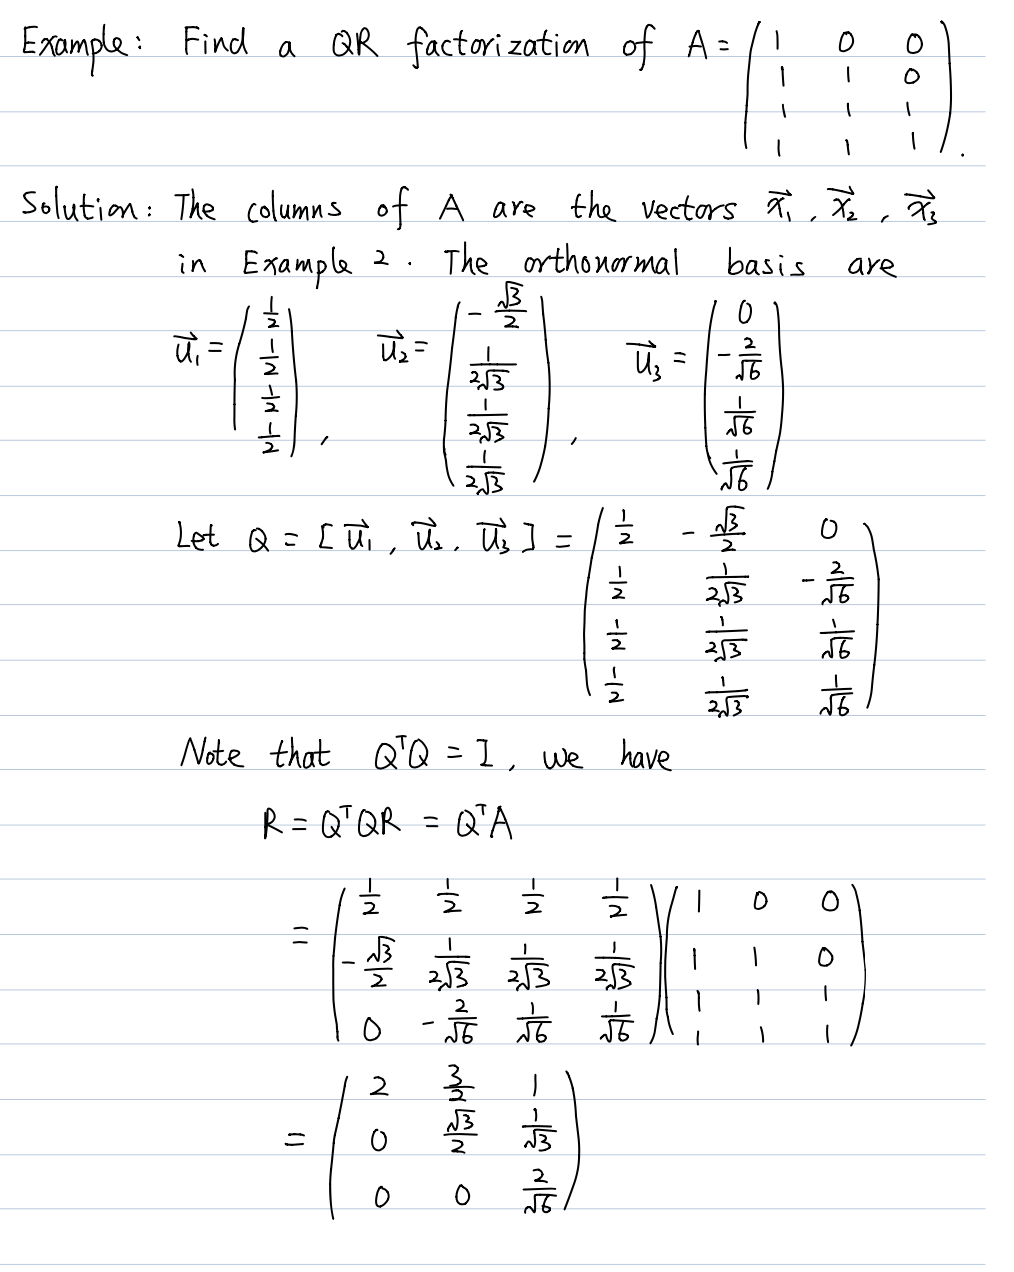
\includegraphics[width = .5\linewidth]{Revision3}
\end{figure}


\subsection{Least-Square Problems}
General least-squares problem: To find an $\hat{\vec{x}}$ that makes $\norm{\vec{b}- A\hat{\vec{x}}}$ as small as possible.

Definition: If $A$ is $m\times n$ and $\vec{b}$ is in $\mathbb{R}^m$, a least-squares solution of $A\vec{x} = \vec{b}$ is an $\hat{\vec{x}}$ in $\mathbb{R}^n$ such that $$\norm{\vec{b}- A\hat{\vec{x}}} \leq \norm{\vec{b}- A\vec{x}}$$
for all $\vec{x}$ in $\mathbb{R}^n$.

Theorem: The set of least-squares solutions of $A\vec{x} = \vec{b}$ coincides with the nonempty set of solutions of the normal equations $$A^TA\vec{x} = A^T\vec{b}$$

Theorem: Let $A$ be an $m\times n$ matrix. The following statements are logically equivalent:
\begin{enumerate}
    \item The equation $A\vec{x} = \vec{b}$ has a unique least-squares solution for each $\vec{b}$ in $\mathbb{R}^m$.
    \item The columns of $A$ are linearly independent.
    \item The matrix $A^TA$ is invertible.
\end{enumerate}


For given $A$ and $\vec{b}$, $\hat{\vec{x}} = \begin{pmatrix}
    \dfrac{\vec{b}\cdot\vec{a_1}}{\vec{a_1}\cdot\vec{a_1}} \\
    \dfrac{\vec{b}\cdot\vec{a_2}}{\vec{a_2}\cdot\vec{a_2}}
\end{pmatrix}$

Theorem: Given an $m\times n$ matrix $A$ with linearly independent columns, let $A = QR$ be a $QR$ factorization of $A$. Then, for each $\vec{b}$ in $\mathbb{R}^m$, the equation $A\vec{x} = \vec{b}$ has a unique least-squares solution, given by $$\hat{\vec{x}} = R^{-1}Q^T\vec{b}$$
$$R\vec{x} = Q^T\vec{b}$$




\subsection{Applications to Linear Models}



\section{Chapter 7}
\subsection{Diagonalization of Symmetric Matrices}
\subsection{Quadratic Form}



\end{document} 